\setcounter{chapter}{2}
\chapter{PRÉPARATION AU LANCEMENT}
\minitoc %insert la minitoc
\graphicspath{{Chapitre3/figures/}}

%\DoPToC

%==============================================================================
\pagestyle{fancy}
\fancyhf{}
\fancyhead[R]{\bfseries\rightmark}
\fancyfoot[R]{\thepage}
\renewcommand{\headrulewidth}{0.5pt}
\renewcommand{\footrulewidth}{0pt}
\renewcommand{\chaptermark}[1]{\markboth{\MakeUppercase{\chaptername~\thechapter. #1 }}{}}
\renewcommand{\sectionmark}[1]{\markright{\thechapter.\thesection~ #1}}

\begin{spacing}{1.5}

%==============================================================================
\section*{Introduction}
Avant d'appréhender le développment du système, il est primordial d'acquérir une compréhension claire des besoins des parties prenantes au projet, et des fonctionalités escomptées du système.\\
Ce chapitre couronne l'étape d'élaboration de la vision de notre produit, par la spécification des besoins. La phase d'inception se poursuit avec l'édification de l'architecture globale du produit et le choix de l'environnement technique. Ces deux parties conclueront le chapitre et annoncent l'achèvement de la phase d'inception.

%==============================================================================
\section{Analyse des besoins}
L'analyse des besoins a pour objectif l'identification des acteurs du système et de leurs rôles, ainsi que la spécification des besoins et des contraintes contre lesquelles le produit final sera validé. Il existe deux types de besoins :
\begin{itemize}
    \item Les besoisn fonctionnels, qui présentent ce que l'utilisateur attend en terme de service
    \item Les besoins non fonctionnels, qui présentent les contraintes sous lesquelles l'application doit être opérationnelle
\end{itemize}

%-----------------------------------------------------------------------------------
\subsection{Objet global du projet}
L'objectif du projet consiste à la conception, au développement, ainsi qu’au déploiement, d’une application web de gestion de projets, compatible avec tous les terminaux, de format réduit ou large, et disponible d’usage principalement en mode SaaS.\\
Pour toute organisation cliente, l’application permettra essentiellement aux responsables, chefs de projet, de gérer les différents aspects des projets entrepris par leur organisation, ainsi que d’en monitorer l’état.\\

Le produit final comportera ainsi deux parties distinctes :
\begin{itemize}
\item Une application web de gestion de projets en mode SaaS, ou à déploiement en interne
    \item Une solution complémentaire pour la gestion de l’aspect SaaS
\end{itemize}

%-----------------------------------------------------------------------------------
\subsection{Identification des acteurs}
L’application est destinée à être acquise par une organisation de petite ou de grande envergure (entreprise, équipe, …). Au sein de celle-ci, nous pouvons distinguer entre trois types d'acteurs à rôles distincts pour notre système :
\begin{itemize}
    \item \textbf{L'administrateur} : C’est l'utilisateur associé au compte existant par défaut lors de l'acquisition de la solution. Il possède les pleins pouvoirs sur le reste des comptes et a la charge de créer le autres comptes au tout début de la mise en route de l'application.
    \item \textbf{Un chef de projet} : C’est l'utilisateur fondamental du système. Il s'intéresse essentiellement à l'aspect de gestion de projets mais garde la possibilité de créer des comptes utilisateurs, à plus faible ou égal pouvoir, et de les gérer à sa guise.
    \item \textbf{Un intervenant} : Cet utilisateur est généralement externe à l'organisation et a pour but de contribuer à la gestion d'un projet. Son compte est créé par un chef de projet, ou l'administrateur, lequel lui procure des droits d'accès à différentes parties d'un projet, son rôle se restraignant à intervenir sur ces parties.
    \item \textbf{Un dirigeant} : Cet utilisateur, généralement interne à l'entreprise, s'intéresse et se limite uniquement à l'exploitation des fonctionalités de reporting offertes par le système, pour l'ensemble du portefeuille de projets. Son compte est créé et géré par l'administrateur.
    \item \textbf{Une partie prenante} : Cet utilisateur se limite à l'exploitation des fonctionalités de reporting offertes par le système dans le cadre d'un projet. Son compte est créé et géré par un chef de projet.
\end{itemize}
\

Pour la solution complémentaire de gestion de l’offre SaaS, on reconnait un type seul acteur, à savoir : L'administrateur SaaS. C’est lui qui gère les clients de l’offre SaaS. Il a la charge de monitorer l’usage de l’application en mode SaaS et de remédier aux requêtes des clients.

%-----------------------------------------------------------------------------------
\subsection{Spécification fonctionnelles}
On énumère ici les différentes contraintes et besoins fonctionnels requis de la part du livrable final.\\
L’application doit être en mesure d’offrir les fonctionnalités suivantes :
\begin{itemize}
    \item \textbf{Gestion du portefeuille de projets} : L'ensemble des projets du client doit être regoupé sous un portefeuille, qui offre des fonctionalités d'ajout et d'édition d'un ou plusieurs projets.
    \item \textbf{Gestion de la charte d'un projet} : Il s'agit d'offrir à l'utilisateur la possibilité de fournir les détails relatifs à la charte d'un projet dès sa création, tout en gardant la possibilité d'en éditer le contenu à postériori.
    \item \textbf{Reporting au niveau projet} : Une vue d'ensemble de l'état global d'un projet doit être accessible au travers d'un tableau de bord, contenant un agencement d'indicateurs clés pour le pilotage d'un projet.
    \item \textbf{Gestion de l'intégration} : Un projet doit pouvoir être structuré sous les différents niveaux suivants : projet, sous projet et chantier. Un projet peut inclure un ensemble de sous projets ou de chantiers, directemnt ratachés à lui. Un sous projet existe uniquement sous un projet, et peut lui-même contenir une multitude de chantiers, lui étant directement associés.
    \item \textbf{Gestion du plan d'action} : Une action est une tâche à réaliser, disposant essentiellement d'une description, d'un responsable et d'une date de clôture planifiée. Une action doit pouvoir être rajoutée sous n'importe quel niveau d'un projet, et peut être mise à jour ou bien supprimée. Un indicateur sur les actions en retard sera mis à disposition.
    \item \textbf{Gestion des coûts} : Le budget d'un projet ou d'un sous projet peut être renseigné et mis à jour tout au long de son existance. La gestion du budget inclut la spécification du budget initial, du buget consommé ainsi que d'une estimation du budget qui reste à consommer. Elle offre par ailleurs un indicateur sur le budget total prévisonnel.
    \item \textbf{Gestion du reste à faire} : Un reste à faire se distingue par une description et une charge associée, en homme / jour. Les restes à faire peuvent être créés et mis à jour, et sont rattachables à n'importe quel niveau d'un projet.
    \item \textbf{Planification} : La planification d'un projet ou d'un sous projet sera possible au travers de la création et de la consultation ultérieure des principaux jalons du niveau de projet. En essence, un jalon est défini par une brève description associée à une date d'échéance.
    \item \textbf{Gestion du "Scope"} : La gestion du "scope" ou du périmètre d'un niveau de projet s'accomplit principalement via la fourniture de documents en pièces jointes au niveau en question. D'autre part, la gestion du périmètre couvre la gestion du changement et des points en suspens. Un point en suspens est un point relatif au niveau de projet, en attente de résolution, auquel un responsable est assigné. La gestion du changement quant à elle est formalisée au travers de la soumission de demandes de changement. Chaque demande inclut essentiellement le demandeur ainsi que la décision prise par rapport à celle-ci.
    \item \textbf{Gestion des risques} : Le définition des risques peut être réalisée à n'importe quel niveau d'un projet. Un risque est défini par une description du risque encouru, associée à une probabilité et un impact. Ces derniers sont utilisés pour générer un indicateur sur le niveau de criticité (KRI \ref{ANGRAMME}) du risque. Leur suivi est réalisé principalement au travers de la spécification du statut, du plan d'action et des dispositions à prendre pour chaque risque, ainsi que d'une date de qualification et une date de clôture.
    \item \textbf{Gestion des ressources humaines} : La définition des ressources humaines peut être réalisée au niveau du portefeuille global de projets ou bien au niveau d'un projet ou d'un sous projet. Les ressources globales peuvent plus tard être assignées à un projet en particulier. Au sein d'un projet ou d'un sous projet, les ressources humaines peuvent être renseignées, mises à jour, et éventuellement assignées à une action ou un point en suspens. Une ressource humaine peut également être assignée en tant que responsable d'un plan de communication au niveau d'un projet.
    \item \textbf{Gestion de la communication} : La gestion de la communication se déroule au sein d'un projet. Elle inclut la définition de plans de communication, se distinguant par une description et un responsable communication, de même que la planification de réunions, disposant chacune d'un nom, d'une date et d'un lieu, acoompagnés d'un statut, ainsi que des comptes rendus de réunions.
    \item \textbf{Gestion des ressources non humaines} : Toute ressource matérielle ou immatérielle associée à un niveau de projet doit pouvoir être renseignée et mise à jour.
    \item \textbf{Publication de mises à jour} : L'état d'un projet doit pouvoir être archivé sous forme d'une mise à jour.
\end{itemize}
\

D'autre part, la solution adjointe de gestion du service SaaS devra quant à elle permettre de gérer les clients de l'offre SaaS : création d’un client, mise à jour des détails associées à un client et gestion du compte administrateur attaché.

%-----------------------------------------------------------------------------------
\subsection{Spécification non fonctionnelles}
En plus d’apporter les fonctionnalités citées précédemment, le produit final devra être en mesure d'assurer les aspects suivants :
\begin{itemize}
    \item \textbf{Sécurité} :
        \begin{itemize}
            \item[•] Isoler proprement les données des clients, et limiter efficacement leurs accès d'un client à un autre.
            \item[•] Mettre en place un système d’authentification et d’autorisation robuste.
        \end{itemize}
    \item \textbf{Performance} : Être réactive et relativement rapide lors de l'exécution.
    \item \textbf{Ergonomie} : Offrir une interface conviviale, intuitive et facile d’usage pour tous les types de dispositifs supportés.
    \item \textbf{Fiabilité} :
        \begin{itemize}
            \item[•] Conserver un comportement cohérent tout au long de la durée d'utilisation.
            \item[•] Éviter toute perte de donnée non intentionnelle.
            \item[•] Éviter ou résoudre les conflits engendrés par l’utilisation concurrente.
        \end{itemize}
    \item \textbf{Compatibilité} : Supporter la majorité des dispositifs des utilisateurs (smartphones, tablettes, ordinateurs, …) de manière adaptée à chacun.
    \item \textbf{Journalisation} :
        \begin{itemize}
            \item[•] Logging des événement importants.
            \item[•] Historiser l'état d'un projet et de ses mises à jour.
        \end{itemize}
\end{itemize}

%-----------------------------------------------------------------------------------
\subsection{Diagramme de cas d'utilisations}
La figure \ref{fig:useCasesDiag} illustre le diagramme de cas d'utilisation global de l'application. Il offre une représentation globale des principaux services offerts par le système, en fonction du type d'utilisateur.

\begin{figure}[H]
\centering
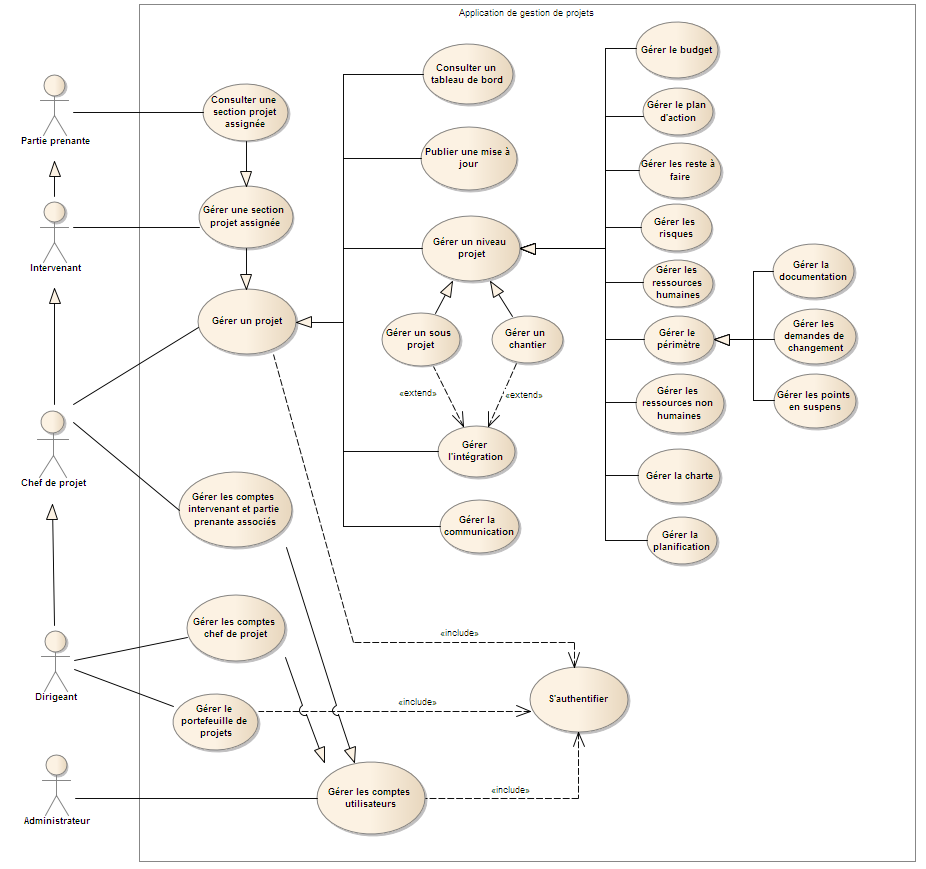
\includegraphics[width=1\linewidth]{useCasesDiag.png}
\caption{Diagramme global de cas d'utilisation}
\label{fig:useCasesDiag}
\end{figure}


%==============================================================================
\section{Architecture générale}

%-----------------------------------------------------------------------------------
%\subsection{}


%==============================================================================
\section{Choix techniques}


%==============================================================================
\section*{Conclusion}
Le dénouement de la phase d'inception annonce le début de la phase de construction.

%==============================================================================
\end{spacing}
